\section{Background}\label{sec:background}

In this section, we introduce the theoretical foundations of hybrid systems, namely the hybrid automata. We then give a brief introduction to PDDL2.1 and then explain how it is extended to describe the hybrid automata in PDDL+. After this we introduce planning as Boolean Satisfiability and then SMT.

\subsection{Hybrid Systems}

A hybrid system is a system where there are both continuous variables and discrete logical modes of operation. It represents a powerful model to describe the dynamic behaviour of modern engineering artefacts. %Hybrid systems frequently occur in practice, e.g., in robotics or embedded systems. 
%Dealing with hybrid systems is becoming more and more an important challenge, as many real-world scenarios feature a mixture of discrete and continuous behaviours. Some example applications include coordination of activities of a planetary lander, oil refinery management, autonomous vehicles, chemical plant management~\cite{chemical}, planning for smart grids~\cite{ucp}, and battery management~\cite{battery}. Such scenarios motivate the need to reason with mixed discrete-continuous domains.

The theory of hybrid automata, introduced by Henzinger~\cite{henzinger}, represents a well-defined formalism for describing hybrid systems. Intuitively, hybrid automata are finite state automata extended with continuous variables that evolve over time. More formally, we have the following:

\begin{definition}[Hybrid Automaton]\label{def:ha}
A \emph{hybrid automaton} is a tuple $\ha=(\loc,\var,\Hinit,\relc,\reld,\inv)$, where 
\begin{itemize}
\item \loc\ is a finite set of locations,
\item $\var=\{x_1, \dots, x_n\}$ is a set of real-valued variables,
\item $\Hinit(\ell)\subseteq\RealUniverse$ is the set of initial values for $x_1,\dots,x_n$ for all locations $\ell$.
\item For each location $\ell$, $\relc(\ell)$ is a relation over the variables in \var\ and their derivatives of the form:
\[ \dot{x}(t) = Ax(t)+u(t), u(t) \in \Input, \]
where $x(t)\in \RealUniverse$, $A$ is a real-valued $n \times n$ matrix and $\Input \subseteq \RealUniverse$ is a closed and bounded convex set.
\item \reld\ is a set of discrete transitions. A discrete transition $t\in\reld$ is defined as a tuple $(\ell,\guard,\update,\ell')$ where $\ell$ and $\ell'$ are the source and the target locations, respectively, $\guard$ is the guard of $t$ (given as a linear constraint), and $\update$ is the update of $t$ (given by an affine mapping).
\item $\inv(\ell)\subseteq\RealUniverse$ is an invariant for all locations $\ell$. 
\end{itemize}
\end{definition}

An example is the hybrid automaton for a thermostat shown in Figure~\ref{fig:thermostat}. Here, the temperature is represented by the continuous variable $x$. In the discrete location corresponding to the heater being off, the temperature falls according to the flow condition $\dot{x}=-0.1x$, while, when the heater is on, the temperature increases according to the flow condition $\dot{x}=5-0.1x$. The discrete transitions state that the heater \textit{may} be switched on when the temperature falls below 19 degrees, and switched off when the temperature is greater than 21 degrees. Finally, the invariants state that the heater can be on (off) \textit{only} if the temperature is not greater than 22 degrees (not less than 18 degrees).

% THERMOSTAT HYBRID AUTOMATA
\begin{figure*}[htb]
\centering
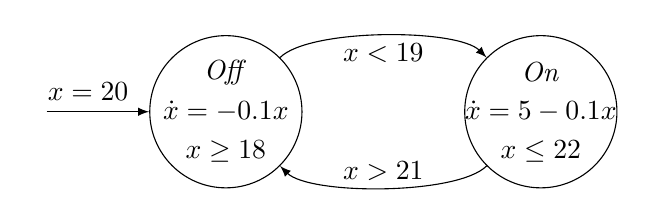
\begin{tikzpicture}[>=latex]
   
  \begin{scope}

%   \draw  (1,1) rectangle (7,1.5);

%\filldraw[black] (0,0) circle (2pt) node[anchor=west] {s};

  \node[circle, inner sep=2pt,draw, minimum height=55pt] (p1) at (-4,0) {};
      \node (p0_d) at (-4.0,0.5) {\textit{Off}};
      \node (p0_d) at (-4.0,0) {$\dot{x}=-0.1x$};
      \node (p0_d) at (-4.0,-0.5) {$x \geq 18$};
  
  \node[circle, inner sep=2pt,draw, minimum height=55pt] (p2) at (0,0) {};
      \node (p0_d) at (0.0,0.5) {\textit{On}};
      \node (p0_d) at (0.0,0) {$\dot{x}=5-0.1x$};
      \node (p0_d) at (0.0,-0.5) {$x \leq 22$};
  
     \draw[->] (p1) .. controls +(45:1.5) and +(135:1.5) .. (p2);
     \node (p0_d) at (-2.0,-0.75) {$x > 21$};
     
      \draw[->] (p2) .. controls +(-135:1.5) and +(-45:1.5) .. (p1);
      \node (p0_d) at (-2.0,0.75) {$x < 19$};
      
      
      \node (p0t) at (-5.75,0.25) {$x=20$};
      \node (p0) at (-6.40,-0.0) {};
        \draw[->] (p0) edge (p1);  
      
%       \draw[->] (p2) edge [loop right] node {} (p2);  
     
%     \node[circle, inner sep=2pt,draw, minimum height=20pt](p3) at (0.25,3) {on}; 
%     \node[circle, inner sep=2pt,draw, minimum height=20pt](p4) at (-0.5,1.5) {$\text{int}_2$}; 
%     
%     \node (p0_d) at (1.2,0) {$\inv:\dot T=0$};

  
%   \node (p0_d) at (1,1.8) {pre$_{\vdash}\cup$ pre$_{\vdash}^{\num}$};
%   \node (p1_d) at (4,1.8) {pre$_{\leftrightarrow}\cup$ pre$_{\leftrightarrow}^{\num}$};
%   \node (p2_d) at (7,1.8) {pre$_{\dashv}\cup$ pre$_{\dashv}^{\num}$};
% 
%   \node (p3_d) at (1.2,0.7) {eff$_{\vdash}^+\cup$ eff$_{\vdash}^-\cup$ eff$_{\vdash}^{\num}$};
%   \node (p5_d) at (4,0.7) {eff$_{\leftrightarrow}^{\num}$};
%   \node (p6_d) at (6.8,0.7) {eff$_{\dashv}^+\cup$ eff$_{\dashv}^-\cup$ eff$_{\dashv}^{\num}$};
% 
%     \node (p7_d) at (4,1.25) {$A$};
%   
  \end{scope}
\end{tikzpicture}
\caption{Thermostat hybrid automaton}
\label{fig:thermostat}
\end{figure*}

\subsection{PDDL2.1 and PDDL+ Planning}

Application of planners in real world problems has challenged the limitations of PDDL and increased the necessity of dealing with time and resources. This lead to the development of PDDL2.1~\cite{fox03} as the extension of PDDL able to model temporal domains. PDDL2.1 has been extended to PDDL+~\cite{pddl+} to enable the modelling of mixed discrete-continuous domains. In this section we first discuss the semantics of PDDL2.1 and later describe the extensions that have been added in PDDL+.

\begin{definition}[PDDL2.1 Planning]\label{def:pddl21}
A PDDL2.1 planning problem is a tuple $\Pi:=\{P,V,A,I,G\}$, where $P$ is a set of propositions; $V$ is a vector of real variables, called fluents; both are manipulated by $A$, a set of durative and instantaneous actions.
$I(P,V)$ is a function over $P\cup V$ which describes the \textit{initial state} of the problem and $G(P,V)$ is a function that describes the \textit{goal condition}.
\end{definition}

A durative action $a \in A$ is described as a tuple:
$$
a:=\{pre_{a},\mathit{eff}_{a},dur_{a}\}
$$
where $pre_{a}(P,V)$ is a function over $P\cup V$ that represents the action's preconditions -- conditions that must hold for the action to be applied. Similarly, $\mathit{eff}_{a}$ represents the action's effects, and $dur_{a}$ is a duration constraint, a conjunction of numeric constraints corresponding to the duration of the action $a$.

A single condition is either a single proposition $p\in P$, its negation, or a numeric constraint over $V$. A precondition is a conjunction of zero or more single conditions. The precondition of an action $pre_a$ can be separated into three disjoint subsets:
$$
pre_{\vdash a}, pre_{\leftrightarrow a}, pre_{\dashv a}\subseteq pre_{a}
$$
These represent the conditions that must hold at the start of the action, throughout its execution, and at the end of the action, respectively.

Action effects are described by seven subsets:
$$
\begin{array}{l}
\mathit{eff}^{+}_{\vdash a},\,\mathit{eff}^{-}_{\vdash a},\,\mathit{eff}^{num}_{\vdash a}, \\
\mathit{eff}^{+}_{\dashv a},\,\mathit{eff}^{-}_{\dashv a},\,\mathit{eff}^{num}_{\dashv a}, \\
\mathit{eff}_{\leftrightarrow a}
\end{array}
$$
The first six are the instantaneous effect of adding or removing propositions, or instantaneous numeric effects. These are bound to the start or end of the action. For example, $\mathit{eff}^{+}_{\vdash a}$ denotes the propositions added at the start of the action. In the semantics of PDDL2.1, the values of such instantaneous effects can be exploited to support other actions only after a small amount of time $\epsilon$~\cite{fox03}. This is referred to as \textit{epsilon separation}. The final set, $\mathit{eff}_{\leftrightarrow a}$ is a conjunction of \textit{continuous} numeric effects $\mathit{eff}_{\leftrightarrow}$, which are applied continuously while the action is executing. As a special case, \textit{instantaneous} actions have duration $0$, have only one set of preconditions $pre_a$; and three sets of effects $\mathit{eff}^{+}_a$, $\mathit{eff}^{-}_a$, and $\mathit{eff}^{num}_a$.

Actions can only be applied together at the same time if they are not mutually exclusive (mutex). Actions $a1$ and $a2$ can be applied simultaneously if:
$$
\begin{array}{c}
pre_{a1} \cap (\mathit{eff}^{+}_{a2} \cup \mathit{eff}^{-}_{a2} \cup \mathit{eff}^{num}_{a2}) = \emptyset \\
\mathit{eff}^{+}_{a1} \cap \mathit{eff}^{-}_{a2} = \mathit{eff}^{+}_{a2} \cap \mathit{eff}^{-}_{a1} = \emptyset \\
\{v1 \in \mathit{eff}^{num}_{a1}\} \cap \{v2 \in \mathit{eff}^{num}_{a2}\} = \emptyset \\
\end{array}
$$

PDDL+ is an extension of PDDL2.1, based on hybrid automata semantics. PDDL+ extends PDDL2.1 to support the modelling of exogenous events, reflecting changes that are initiated by the environment. These are introduced by the new constructs of \textit{processes} and \textit{events}.

\begin{definition}[PDDL+ Planning]\label{def:pddl+}
A PDDL+ planning problem is a tuple $\Pi+:=\big \langle P,V,A,Ps,E,I,G\big \rangle $, in which $P$ is a set of propositions; $V$ is a vector of real variables, called fluents; and $A$ is a set of durative and instantaneous actions. $Ps$ is a set of processes, and $E$ a set of events. $I(P,V)$ and $G(P,V)$ represent the initial state and goal condition respectively.
\end{definition}

The elements $P,V,A,I$, and $G$ are as in Definition~\ref{def:pddl21}. As an analogue, an event $e\in E$ is akin to an instantaneous action: if an event's preconditions $pre_e$ are satisfied, it occurs, yielding the event's instantaneous effects. Similarly, processes are akin to durative actions which apply continuous effects over a period of time.

Note that continuous processes are triggered as soon as their precondition becomes true, and in this sense they \textit{must} be triggered. Exogenous events follow the same semantics. The rationale behind this is that processes and events are used to model changes that are initiated by changes in the world, therefore they are not under the direct control of the executive and are triggered immediately (see Bogomolov et al.~\cite{bogomolov14} for more details). This is a critical distinction between processes/events and actions. The process/event will automatically occur as soon as its precondition is satisfied; whereas an action will only happen if chosen to be executed by the planner.

Furthermore, effects become instantaneously available to events, without the epsilon separation. This means, if one event $e1$ is triggered, with effects that satisfy another event $e2$ and trigger a process $p1$, then $e1$, $e2$, and the start of $p1$ all happen at exactly the same time-point. It is due to this behaviour that PDDL+ semantics place a bound on the number of cascading (parallel) events. According to PDDL+ semantics, a causal chain of events cannot include a cycle, and a single event cannot be triggered more than once in a single instant~\cite{fox2002pddl+}.

Given the PDDL+ semantics for modelling hybrid systems, finding an efficient planner that can handle events and processes is the next crucial step. A number of methods have been proposed to handle mixed discrete and continuous domains. We review these in Section~\ref{sec:related_work}.

\subsection{Planning as Satisfiability}

The problem of determining Boolean Satisfiability Problem (SAT) is the problem of finding an assignment of truth values to variables in order to make a set of propositional formulae true. The problem is stated as: given a Boolean expression $\phi$ with variables $X: \{ x_1, x_2, ... , x_n\}$, there exists an assignment to variables $X$ such that $\phi$ is satisfied? In other words:
$$
\exists \, x_1, x_2, ... , x_n \quad\phi?
$$
For example,
$$
\phi := (\neg x_1 \vee \neg x_2) \wedge (x_1 \vee x_3) \wedge (x_3 \vee x_2) \wedge \neg x_3
$$
is false, since there are no assignments to the three variables $x_1, x_2, x_3$ that will satisfy $\phi$.
%
In the context of planning, we are focusing on SAT solvers that solve the decision problem and if the expression is satisfiable, return an example satisfying assignment. Kautz and Selman~\cite{kau92} formalised propositional planning as a Boolean Satisfiability (SAT) problem in the following way.

First, the classical planning problem for a fixed horizon $n$ is modelled by defining $n$ copies of the Boolean variables which describe the state and actions, and unrolling $n$ times the transition relation that holds between states. This gives a set of variables ($X$) and constraints between them ($\phi$). A satisfying assignment to the variables corresponds to a plan trace.

In more detail, the set of variables $X$ comprises one Boolean variable for each $a\in A$, and each $p\in P$ \footnote{Similar to Definition~\ref{def:pddl21}, in classical planning we have a set of actions and a set of propositions which are shown as $A$ and $P$, respectively.} at each time-step $t_0, \ldots, t_n$. In propositional planning, there are no numeric variables $v\in V$. Constraints are added to $\phi$, asserting:
\begin{itemize}
\item The initial state holds at time-step $0$, and goals at time-step $n$.
\item If an action is true, then its preconditions hold in that time-step.
\item If an action is true, then its effects hold in the following time-step.
\item Two actions that are mutex cannot be applied together in the same time-step.
\end{itemize}

To solve the original planning problem without a fixed time horizon, an initial encoding with horizon $n_0$ is solved, and if found, the satisfying assignment is converted into a corresponding plan. Otherwise, the horizon is incremented and the process is repeated~\cite{kau99}.

A significant number of works have been devoted to formalising planning problems using propositional logic, and improving those encodings~\cite{rin06,che07,rob09,rin10,cas12b}, which we discuss in Section~\ref{sec:related_work}.

\subsection{Satisfiability Modulo Theory}

Satisfiability Modulo Theory (SMT)~\cite{bar18} is the problem of deciding the satisfiability of a first-order formula expressed in a given theory. An SMT problem is given as a set of variables and a set of constraints over those variables. In contrast to the SAT problem, the variables are not restricted to Boolean values, but depend upon a \textit{theory}, and the constraints are expressed with respect to a background \textit{logic}.
%
The theory and logic are critical elements of an SMT problem. Theories exist for Boolean propositions, finite and infinite trees, lists, bitvectors, arrays, integers, and reals. SMT takes advantage of the fact that some of them already have efficient solvers in order to reason more efficiently. In our work we use the theory of real numbers and the logic of \textit{quantifier-free non-linear real arithmetic}.

For example, an SMT problem in \textit{quantifier-free linear real arithmetic} might be:

$$
\exists u,v,x,y,z\quad\phi?
$$
where
$$
\phi:= (x+3 <= 2u) \vee (v+4 >= y) \vee (x+y+z >= 2)
$$

Problems in SMT can be expressed in the SMT-LIB standard syntax~\cite{bar10}. Figure~\ref{fig:smtlib} illustrates the example problem above in the standard sytax. The encoding we describe in this paper is produced in this standard format, and can be read many SMT solvers, including {\sc z3}~\cite{dem08}, which we use to solve our problems in Section~\ref{sec:experiments}. 

\begin{figure}[htb]
\centering
\begin{BVerbatim}
( set-logic QF_LRA )
( declare-fun u () Real)
( declare-fun v () Real)
( declare-fun x () Real)
( declare-fun y () Real)
( declare-fun z () Real)
( assert
    (or
    ( <= (+ x 3) (* 2 u ) )
    ( >= (+ v 4) y )
    ( >= (+ x y z ) 2)
    )
)
\end{BVerbatim}
\caption{SMT problem in the SMT-LIB standard syntax.}
\label{fig:smtlib}
\end{figure}
